%% LyX 2.4.1 created this file.  For more info, see https://www.lyx.org/.
%% Do not edit unless you really know what you are doing.
\documentclass[journal,article,submit,pdftex,moreauthors]{Definitions/mdpi}
\usepackage{textcomp}
\usepackage[utf8]{inputenc}
\usepackage{float}
\usepackage{url}
\usepackage{graphicx}

\makeatletter

%%%%%%%%%%%%%%%%%%%%%%%%%%%%%% LyX specific LaTeX commands.

\Title{Predicting the damage of urban fires with Grammatical Evolution.}

\TitleCitation{Predicting the damage of urban fires with Grammatical Evolution}

\Author{Constantina Kopitsa$^{1}$, Ioannis G. Tsoulos$^{2,*}$, Andreas Miltiadous$^{3},$Vasileios
Charilogis$^{4}$}

\AuthorNames{Kopitsa, C., Tsoulos, I.G., Miltiadous, A, Charilogis, V.}

\AuthorNames{Constantina Kopitsa, Ioannis Tsoulos, Andreas Miltiadous and Vasileios
Charilogis.}

\AuthorCitation{Kopitsa, C.; Tsoulos, I.G.; Miltiadous, A., Charilogis, V. }


\address{$^{1}$\quad{}Department of Informatics and Telecommunications,
University of Ioannina, Greece;k.kopitsa@uoi.gr\\
$^{2}$\quad{}Department of Informatics and Telecommunications, University
of Ioannina, Greece; itsoulos@uoi.gr\\
$^{3}\quad$Department of Informatics and Telecommunications, University
of Ioannina, Greece; a.miltiadous@uoi.gr\\
$^{4}\quad$Department of Informatics and Telecommunications, University
of Ioannina, Greece; v.charilog@uoi.gr}


\corres{Correspondence: itsoulos@uoi.gr}


\abstract{Fire, whether wild or urban, depends on the triad of oxygen, fuel,
and heat. Urban fires, though smaller in scale, have devastating impacts,
as evidenced by the 2018 wildfire in Mati, Attica (Greece), which
claimed 104 lives. The elderly and children are the most vulnerable
due to mobility and cognitive limitations. This study applies Grammatical
Evolution (GE), a machine learning method that generates interpretable
classification rules to predict the consequences of urban fires. Using
historical data (casualties, containment time, meteorological/demographic
parameters), GE produces classification rules in human readable form.
The rules achieve over 85\% accuracy, revealing critical correlations.
For example, high temperatures (\textgreater 35°C) combined with
irregular building layouts exponentially increase fatality risks,
while firefighter response time proves more critical than fire intensity
itself. Applications include dynamic evacuation strategies (real-time
adaptation), preventive urban planning (fire-resistant materials,
green buffer zones), and targeted awareness campaigns for at-risk
groups.Unlike \textquotedbl black-box\textquotedbl{} machine learning
techniques, GE offers transparent, human-readable rules, enabling
firefighters and authorities to make rapid, informed decisions. Future
advancements could integrate real-time data (IoT sensors, satellites)
and extend the methodology to other natural disasters. Protecting
urban centers from fires is not only a technological challenge but
also a moral imperative to safeguard human lives and societal cohesion.}


\keyword{Urban fires; Machine learning; Neural networks; Genetic Programming;
Grammatical Evolution.}

\DeclareTextSymbolDefault{\textquotedbl}{T1}
%% Because html converters don't know tabularnewline
\providecommand{\tabularnewline}{\\}

%%%%%%%%%%%%%%%%%%%%%%%%%%%%%% Textclass specific LaTeX commands.
\newenvironment{lyxcode}
	{\par\begin{list}{}{
		\setlength{\rightmargin}{\leftmargin}
		\setlength{\listparindent}{0pt}% needed for AMS classes
		\raggedright
		\setlength{\itemsep}{0pt}
		\setlength{\parsep}{0pt}
		\normalfont\ttfamily}%
	 \item[]}
	{\end{list}}

%%%%%%%%%%%%%%%%%%%%%%%%%%%%%% User specified LaTeX commands.
%  LaTeX support: latex@mdpi.com 
%  For support, please attach all files needed for compiling as well as the log file, and specify your operating system, LaTeX version, and LaTeX editor.

%=================================================================
%\documentclass[preprints,article,submit,pdftex,moreauthors]{Definitions/mdpi} 
% For posting an early version of this manuscript as a preprint, you may use "preprints" as the journal. Changing "submit" to "accept" before posting will remove line numbers.

% Below journals will use APA reference format:
% admsci, behavsci, businesses, econometrics, economies, education, ejihpe, famsci, games, humans, ijcs, ijfs, journalmedia, jrfm, languages, psycholint, publications, tourismhosp, youth

% Below journals will use Chicago reference format:
% arts, genealogy, histories, humanities, jintelligence, laws, literature, religions, risks, socsci

%--------------------
% Class Options:
%--------------------
%----------
% journal
%----------
% Choose between the following MDPI journals:
% accountaudit, acoustics, actuators, addictions, adhesives, admsci, adolescents, aerobiology, aerospace, agriculture, agriengineering, agrochemicals, agronomy, ai, air, algorithms, allergies, alloys, amh, analytica, analytics, anatomia, anesthres, animals, antibiotics, antibodies, antioxidants, applbiosci, appliedchem, appliedmath, appliedphys, applmech, applmicrobiol, applnano, applsci, aquacj, architecture, arm, arthropoda, arts, asc, asi, astronomy, atmosphere, atoms, audiolres, automation, axioms, bacteria, batteries, bdcc, behavsci, beverages, biochem, bioengineering, biologics, biology, biomass, biomechanics, biomed, biomedicines, biomedinformatics, biomimetics, biomolecules, biophysica, biosensors, biosphere, biotech, birds, blockchains, bloods, blsf, brainsci, breath, buildings, businesses, cancers, carbon, cardiogenetics, catalysts, cells, ceramics, challenges, chemengineering, chemistry, chemosensors, chemproc, children, chips, cimb, civileng, cleantechnol, climate, clinbioenerg, clinpract, clockssleep, cmd, cmtr, coasts, coatings, colloids, colorants, commodities, complications, compounds, computation, computers, condensedmatter, conservation, constrmater, cosmetics, covid, crops, cryo, cryptography, crystals, csmf, ctn, curroncol, cyber, dairy, data, ddc, dentistry, dermato, dermatopathology, designs, devices, diabetology, diagnostics, dietetics, digital, disabilities, diseases, diversity, dna, drones, dynamics, earth, ebj, ecm, ecologies, econometrics, economies, education, eesp, ejihpe, electricity, electrochem, electronicmat, electronics, encyclopedia, endocrines, energies, eng, engproc, ent, entomology, entropy, environments, epidemiologia, epigenomes, esa, est, famsci, fermentation, fibers, fintech, fire, fishes, fluids, foods, forecasting, forensicsci, forests, fossstud, foundations, fractalfract, fuels, future, futureinternet, futureparasites, futurepharmacol, futurephys, futuretransp, galaxies, games, gases, gastroent, gastrointestdisord, gastronomy, gels, genealogy, genes, geographies, geohazards, geomatics, geometry, geosciences, geotechnics, geriatrics, glacies, grasses, greenhealth, gucdd, hardware, hazardousmatters, healthcare, hearts, hemato, hematolrep, heritage, higheredu, highthroughput, histories, horticulturae, hospitals, humanities, humans, hydrobiology, hydrogen, hydrology, hygiene, idr, iic, ijerph, ijfs, ijgi, ijmd, ijms, ijns, ijpb, ijt, ijtm, ijtpp, ime, immuno, informatics, information, infrastructures, inorganics, insects, instruments, inventions, iot, j, jal, jcdd, jcm, jcp, jcs, jcto, jdad, jdb, jeta, jfb, jfmk, jimaging, jintelligence, jlpea, jmahp, jmmp, jmms, jmp, jmse, jne, jnt, jof, joitmc, joma, jop, jor, journalmedia, jox, jpbi, jpm, jrfm, jsan, jtaer, jvd, jzbg, kidney, kidneydial, kinasesphosphatases, knowledge, labmed, laboratories, land, languages, laws, life, lights, limnolrev, lipidology, liquids, literature, livers, logics, logistics, lubricants, lymphatics, machines, macromol, magnetism, magnetochemistry, make, marinedrugs, materials, materproc, mathematics, mca, measurements, medicina, medicines, medsci, membranes, merits, metabolites, metals, meteorology, methane, metrics, metrology, micro, microarrays, microbiolres, microelectronics, micromachines, microorganisms, microplastics, microwave, minerals, mining, mmphys, modelling, molbank, molecules, mps, msf, mti, multimedia, muscles, nanoenergyadv, nanomanufacturing, nanomaterials, ncrna, ndt, network, neuroglia, neurolint, neurosci, nitrogen, notspecified, nursrep, nutraceuticals, nutrients, obesities, oceans, ohbm, onco, oncopathology, optics, oral, organics, organoids, osteology, oxygen, parasites, parasitologia, particles, pathogens, pathophysiology, pediatrrep, pets, pharmaceuticals, pharmaceutics, pharmacoepidemiology, pharmacy, philosophies, photochem, photonics, phycology, physchem, physics, physiologia, plants, plasma, platforms, pollutants, polymers, polysaccharides, populations, poultry, powders, preprints, proceedings, processes, prosthesis, proteomes, psf, psych, psychiatryint, psychoactives, psycholint, publications, purification, quantumrep, quaternary, qubs, radiation, reactions, realestate, receptors, recycling, regeneration, religions, remotesensing, reports, reprodmed, resources, rheumato, risks, robotics, rsee, ruminants, safety, sci, scipharm, sclerosis, seeds, sensors, separations, sexes, signals, sinusitis, siuj, skins, smartcities, sna, societies, socsci, software, soilsystems, solar, solids, spectroscj, sports, standards, stats, std, stresses, surfaces, surgeries, suschem, sustainability, symmetry, synbio, systems, tae, targets, taxonomy, technologies, telecom, test, textiles, thalassrep, therapeutics, thermo, timespace, tomography, tourismhosp, toxics, toxins, transplantology, transportation, traumacare, traumas, tropicalmed, universe, urbansci, uro, vaccines, vehicles, venereology, vetsci, vibration, virtualworlds, viruses, vision, waste, water, wem, wevj, wild, wind, women, world, youth, zoonoticdis

%---------
% article
%---------
% The default type of manuscript is "article", but can be replaced by: 
% abstract, addendum, article, book, bookreview, briefreport, casereport, comment, commentary, communication, conferenceproceedings, correction, conferencereport, entry, expressionofconcern, extendedabstract, datadescriptor, editorial, essay, erratum, hypothesis, interestingimage, obituary, opinion, projectreport, reply, retraction, review, perspective, protocol, shortnote, studyprotocol, systematicreview, supfile, technicalnote, viewpoint, guidelines, registeredreport, tutorial
% supfile = supplementary materials

%----------
% submit
%----------
% The class option "submit" will be changed to "accept" by the Editorial Office when the paper is accepted. This will only make changes to the frontpage (e.g., the logo of the journal will get visible), the headings, and the copyright information. Also, line numbering will be removed. Journal info and pagination for accepted papers will also be assigned by the Editorial Office.

%------------------
% moreauthors
%------------------
% If there is only one author the class option oneauthor should be used. Otherwise use the class option moreauthors.

%---------
% pdftex
%---------
% The option pdftex is for use with pdfLaTeX. If eps figures are used, remove the option pdftex and use LaTeX and dvi2pdf.

%=================================================================
% MDPI internal commands - do not modify
\firstpage{1} 
\setcounter{page}{\@firstpage}
\pubvolume{1}
\issuenum{1}
\articlenumber{0}
\pubyear{2025}
\copyrightyear{2025}
%\externaleditor{Firstname Lastname} % More than 1 editor, please add `` and '' before the last editor name
\datereceived{}
\daterevised{ } % Comment out if no revised date
\dateaccepted{}
\datepublished{}
%\datecorrected{} % For corrected papers include a "Corrected: XXX" date in the original paper.
%\dateretracted{} % For retracted papers include a "RETRACTED: XXX" date in the original paper.
\hreflink{https://doi.org/} % If needed use \linebreak
%\doinum{}
%\pdfoutput=1 % Uncommented for upload to arXiv.org
%\CorrStatement{yes}  % For updates
%\longauthorlist{yes} % For many authors that exceed the left citation part

%=================================================================
% Add packages and commands here. The following packages are loaded in our class file: fontenc, inputenc, calc, indentfirst, fancyhdr, graphicx, epstopdf, lastpage, ifthen, lineno, float, amsmath, setspace, enumitem, mathpazo, booktabs, titlesec, etoolbox, tabto, xcolor, soul, multirow, microtype, tikz, totcount, changepage, attrib, upgreek, cleveref, amsthm, hyphenat, natbib, hyperref, footmisc, url, geometry, newfloat, caption

%=================================================================
%% Please use the following mathematics environments: Theorem, Lemma, Corollary, Proposition, Characterization, Property, Problem, Example, ExamplesandDefinitions, Hypothesis, Remark, Definition, Notation, Assumption
%% For proofs, please use the proof environment (the amsthm package is loaded by the MDPI class).

%=================================================================
% The fields PACS, MSC, and JEL may be left empty or commented out if not applicable
%\PACS{J0101}
%\MSC{}
%\JEL{}

%%%%%%%%%%%%%%%%%%%%%%%%%%%%%%%%%%%%%%%%%%
% Only for the journal Diversity
%\LSID{\url{http://}}

%%%%%%%%%%%%%%%%%%%%%%%%%%%%%%%%%%%%%%%%%%
% Only for the journal Applied Sciences:
%\featuredapplication{Authors are encouraged to provide a concise description of the specific application or a potential application of the work. This section is not mandatory.}
%%%%%%%%%%%%%%%%%%%%%%%%%%%%%%%%%%%%%%%%%%

%%%%%%%%%%%%%%%%%%%%%%%%%%%%%%%%%%%%%%%%%%
% Only for the journal Data:
%\dataset{DOI number or link to the deposited data set in cases where the data set is published or set to be published separately. If the data set is submitted and will be published as a supplement to this paper in the journal Data, this field will be filled by the editors of the journal. In this case, please make sure to submit the data set as a supplement when entering your manuscript into our manuscript editorial system.}

%\datasetlicense{license under which the data set is made available (CC0, CC-BY, CC-BY-SA, CC-BY-NC, etc.)}

%%%%%%%%%%%%%%%%%%%%%%%%%%%%%%%%%%%%%%%%%%
% Only for the journal Toxins
%\keycontribution{The breakthroughs or highlights of the manuscript. Authors can write one or two sentences to describe the most important part of the paper.}

%%%%%%%%%%%%%%%%%%%%%%%%%%%%%%%%%%%%%%%%%%
% Only for the journal Encyclopedia
%\encyclopediadef{Instead of the abstract}
%\entrylink{The Link to this entry published on the encyclopedia platform.}
%%%%%%%%%%%%%%%%%%%%%%%%%%%%%%%%%%%%%%%%%%

%%%%%%%%%%%%%%%%%%%%%%%%%%%%%%%%%%%%%%%%%%
% Only for the journal Advances in Respiratory Medicine, Smart Cities and Sensors
%\addhighlights{yes}
%\renewcommand{\addhighlights}{%

%\noindent This is an obligatory section in “Advances in Respiratory Medicine”, whose goal is to increase the discoverability and readability of the article via search engines and other scholars. Highlights should not be a copy of the abstract, but a simple text allowing the reader to quickly and simplified find out what the article is about and what can be cited from it. Each of these parts should be devoted up to 2~bullet points.\vspace{3pt}\\
%\textbf{What are the main findings?}
% \begin{itemize}[labelsep=2.5mm,topsep=-3pt]
% \item First bullet.
% \item Second bullet.
% \end{itemize}\vspace{3pt}
%\textbf{What is the implication of the main finding?}
% \begin{itemize}[labelsep=2.5mm,topsep=-3pt]
% \item First bullet.
% \item Second bullet.
% \end{itemize}
%}
%%%%%%%%%%%%%%%%%%%%%%%%%%%%%%%%%%%%%%%%%%

\makeatother

\begin{document}
\maketitle

\section{Introduction}

Whereas, fires can be triggered by various causes significant fires
are frequently outcome from the following disasters: storms, transportation
accidents, criminal activity / terrorism, droughts, hazardous materials
spills \citep{fire_ref1} and forest fires. Also, Urban fires are
predominantly attributed to negligent cooking practices, whereas rural
fires often stem from faulty electrical installations, malfunctions
in heating systems, or even natural causes such as lightning strikes
\citep{fire_ref2}. Small scale urban fires often do not have a significant
impact on an area, nevertheless on the other hand they still are equally
hazardous to human life, in the socio-economic stability of a community,
or even they contribute to increased insurance premiums \citep{fire_ref1}. 

Referring to human lives, let us examine the numerical data provided
by the Hellenic Fire Service, which is available as open data in accordance
with the European Union Directive (2013/37/EE) aimed at enhancing
transparency \citep{hellenic_fire}. Consequently, as presented in
Figure \ref{fig:graphGreece}, an increase in fatalities associated
with urban fires, has been observed since 2020, with a slight decline
in this trend, in 2023.

\begin{figure}[H]
\begin{centering}
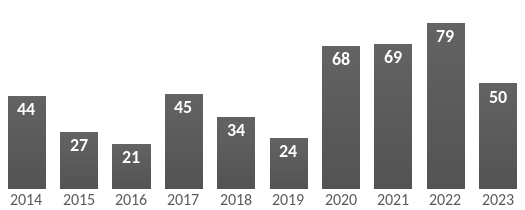
\includegraphics[scale=0.5]{greece_fire_deaths}
\par\end{centering}
\caption{A graph presenting the deaths from fires in Greece for a period from
2014 to 2023.\protect\label{fig:graphGreece}}

\end{figure}
Beyond this, it is observed that in 2018, the human casualties from
the devastating fire in Mati, Attica, have not been accounted for,
as previously mentioned in the Abstract \citep{greek_wikipedia,greek_wildfire}
. This is likely due to the classification of this particular fire
as a wildfire rather than an urban fire.

According to a study conducted, in America, by the National Fire Protection
Association (NFPA), there was an approximate 4\% rise in residential
fires and a 13\% increase in deliberately ignited structural fires
in 2018 \citep{fire_ref2}. Thus, based on the official fire situation
report, Fire Loss in the United States During 2017, published by the
National Fire Protection Association, fire departments across the
United States responded to an estimated 1,319,500 fire incidents in
2017. These incidents led to approximately 3,400 civilian fatalities,
14,670 civilian injuries, and an estimated \$23 billion in direct
property damage \citep{fire_ref2}.

Additionally, the World Health Organization (WHO), an estimated three
million fires occur globally each year, resulting in approximately
180,000 fatalities \citep{who}. Moreover, the majority of these disasters
take place in major urban centers, within low - income countries,
where various economic, social, and environmental factors contribute
to an increased risk of fire incidents . 

Nevertheless, the data demonstrate that wildfires are not solely an
issue confined to low socio-economic status countries. Notably, the
Black Summer of Australia in 2019--2020 remains a significant historical
event. Tragically, the fires claimed 33 lives and impacted thousands
through smoke inhalation and other effects. By the end of the season,
they had burned a record 19 million hectares, destroyed over 3,000
homes, displaced tens of thousands, and caused the loss of billions
of animals \citep{fire_hazards,australian_report}. Furthermore, in
July 2024, wildfires occurred in the Arctic plains of Russia's Far
East, posing significant challenges to containment efforts \citep{fires_siberian,nasa_images}
. That summer, wildfires had already devastated nearly 5 million hectares
of forest in Russia. Wildfires in Russia's Siberian and Far East regions,
which occur annually during the summer, have become more severe in
recent years due to climate change, which has intensified the hot
and dry conditions that fuel these fires \citep{fires_russia}. Climate
change projections, indicate that urban environments may face increasing,
fire hazards \citep{fire_cities}. A stark example of the interconnectedness
between climate change, and wildfires, is evident in the fires that
occurred in Los Angeles in January 2025, and in Japan in February
of the same year. In this connection, Climate scientists are working
to identify the impact of climate change on wildfires. However, the
most substantial human influence may lie in the ignition sources,
as no lightning storms were present at the time, in L.A, to naturally
trigger the fires \citep{fire_climate}. As the relentless wildfire
advanced into urban areas, driven by wind speeds exceeding 80 miles
per hour, it destroyed over 16,000 homes and buildings \citep{fire_climate}.
By February 4, a total of 29 fatalities had been reported \citep{fire_graphics}.
Another technologically and socioeconomically advanced nation, Japan,
was struck by an uncontrolled wildfire on February 26, 2025 \citep{fire_japan}.
The fire scorched over 2,100 hectares and destroyed more than 80 buildings.
Determining whether climate change has directly caused or intensified
specific wildfires is challenging, as other factors, such as land-use
changes, also play a role. However, the IPCC asserts that climate
change is increasing the likelihood of weather conditions that facilitate
the spread of wildfires \citep{fire_bbc}.

From these real events, it is inferred that an unpredictable natural
disaster, such as a wildfire, does not discriminate between low and
high-socioeconomic areas. Furthermore, it highlights the precarious
balance (sword of Damocles) between climate change, and urban expansion
into forested regions. This underscores the critical importance of
our research in predicting the impacts damages of an urban fire. Next,
we will refer to relevant studies focused on the field of urban fire
prediction. A team of researchers, used data from Ankara region, of
Turkey, for analysis of the spatial and temporal patterns of residential
fires, can enable decision-makers to strategically allocate resources
for fire management, based on the intensity of fire clustering over
time and across different locations \citep{fire_turkey}. Next, we
proceed with an article that examines existing research on the social,
economic, and building stock characteristics associated with residential
fire risk in urban neighborhoods \citep{fire_social}. From Australia
in 2010, we have the first study utilizing the Bayesian approach,
to produce detailed spatial forecasts of residential household fires,
across metropolitan South-East Queensland \citep{fire_resident}.
Also, from Australia, a study employs a Markov chain approach to estimate
the likelihood of residential fire occurrences based on historical
fire data. Utilizing fire incident records collected over a decade
in Melbourne, Australia, the spatially integrated fire risk model
forecasts potential fire events by incorporating spatial and temporal
variables as key predictive factors \citep{fire_model}. Subsequently,
the following study builds upon the methodology and effectiveness
of a firefighter-led public education campaign on fire prevention,
which successfully decreased both the frequency, and severity, of
residential structure fires in high-risk areas of Surrey, British
Columbia \citep{fire_freq}. In the sequel, some studies have used
GIS methods, to analyze the fire risk in urban areas. In Turkey, a
study examines fires that have occurred in various locations across
Turkey, including cold storage facilities, factories, and manufacturing
plants. The case data was utilized to calculate risk scores using
Geographic Information System (GIS), Analytical Hierarchy Process
(AHP), and Inverse Distance Weight (IDW) methods \citep{fire_risk_manage}.
In China, in order to select the best suitable fire brigade zone,
they analyze: fire-risk areas, traffic congestion, land cover, and
location. They employ various methods, including Geographic Information
Systems (GIS), Multi-Criteria Decision Making (MCDM), and Location-Allocation
(L-A) techniques, along with multi-source geospatial data such as
land cover, points of interest, drive time, and statistical yearbooks.
Additionally, they used Analytic Hierarchy Processes (AHP) to thoroughly
assess undeveloped areas based on factors such as location, topography,
and potential fire-risk zones \citep{fire_gis}. The next study conducted
in Greece, to develop a fire risk estimation model that integrates
recent land cover changes alongside other critical risk factors. They
implemented a Support Vector Machine (SVM) algorithm \citep{svm}
combined with the Analytic Hierarchy Process (AHP), within a Geographic
Information System (GIS) platform. This approach allowed for a more
precise assessment of fire-prone areas. As a case study, they applied
this methodology to the Dadia-Lefkimi - Soufli National Forest Park,
ensuring a comprehensive evaluation of fire risk in the region \citep{fire_prob}.

Afterwards, a study seeks to assess fire risk in urban areas by analyzing
19 factors related to economic, social, and built environment aspects,
as well as past fire incidents. It employs Multi-Criteria Decision
Making (MCDM) techniques, specifically the Analytic Hierarchy Process
(AHP) to determine the significance and weighting of each criterion.
To illustrate the method’s effectiveness, the research develops an
urban vulnerability index map for Ardabil, Iran, using the Fuzzy-VIKOR
approach within a Geographic Information System (GIS) framework \citep{fire_gis_model}.
Building upon, Analytic Hierarchy Process, the paper from Taiwan,
evaluated the severity of building fires across 17 villages in Taishan
District, New Taipei City. A comprehensive literature review was conducted
to examine the influence of fire severity assessment criteria, which
served as the foundation for identifying key factors, and developing
evaluation items, within the (AHP) framework \citep{fire_big_data}.

Building upon, Analytic Hierarchy Process, the paper from Taiwan,
evaluated the severity of building fires across 17 villages in Taishan
District, New Taipei City. A comprehensive literature review was conducted
to examine the influence of fire severity assessment criteria, which
served as the foundation for identifying key factors, and developing
evaluation items, within the (AHP) framework \citep{fire_safety}.
American researchers, have introduced two machine learning models,
utilizing Random Forest \citep{random_forest1,random_forest2} and
Extreme Gradient Boosting (XGBoost) \citep{xgboost}, to forecast
future service demand in urban areas based on spatial data analysis,
in collaboration with Victoria Fire Department, U.S.A \citep{fire_station}.
A similar study was conducted by Turkish researchers in 2020, and
from China in 2021 \citep{fire_prob}. Specifically, the Turkish colleagues
proposed a group decision-making (GDM) approach, integrating the recently
developed Best--Worst Method (BWM) \citep{bwm}, a multi-criteria
decision-making (MCDM) technique \citep{mcdm}, with Geographic Information
Systems (GIS) to identify optimal locations for new emergency facilities
in Istanbul. Their analysis incorporated the input of two decision-makers
\citep{fire_decision_maker}. Moving forward, another fire risk model
was implemented within the Pittsburgh Bureau of Fire (PBF), and initial
risk models was developed for predicting residential property fire
risk \citep{fire_risk_prediction}.

Furthermore, the subsequent study, is a novel deep sequence learning
model, referred to as the Fire Situation Forecasting Network (FSFN),
is introduced to enhance the processing of information and the analysis
of Spatio -temporal correlations within regional urban fire alarm
datasets \citep{fire_forecast}. Building upon a prior method, on
fire statistics, a weighted fire risk calculation method was developed,
incorporating the frequency of fire occurrences, direct economic losses,
and fire-related casualties. According this approach, and with enhancements
to the K-means clustering algorithm \citep{kmeans}, this study introduced
a fire risk K-means clustering model. This model offers an improved
solution for the automated classification of fire risk levels \citep{fire_stat}.
The next study, seeks to expand the limited empirical research on
urban fires in the Global South by analyzing their causes and dynamics.
Focusing on disaggregated fire incident data from Kathmandu Metropolitan
City (KMC), Nepal, the research identifies key contributing factors
and examines both the spatial and temporal distribution of urban fires
\citep{fire_nepal}. The following study, was conducted in Iran, sought
to apply machine learning algorithms to enhance the accuracy of predicting
firefighting operation duration in urban areas, while also identifying
the key factors that significantly impact this timeframe \citep{fire_ml}.
The subsequent paper, employs an unsupervised deep learning (DL) approach
to categorize hazard levels at fire sites and utilizes an autoregressive
integrated moving average (ARIMA) model to predict temperature variations,
leveraging the extrapolation capabilities of a random forest regressor
\citep{fire_deep}. In the sequel, studies from Japan integrate the
earthquake factor as a cause of urban fires. The following article
introduces the development of a stochastic model designed for time
series forecasting of post-earthquake fire ignitions in buildings,
aiming to enhance post-earthquake fire risk assessment \citep{fire_time_series}.
The same researcher, also developed a physics-based urban fire spread
model that incorporates the stochastic occurrence of spot fires in
the wooden residential areas of Itoigawa City. Utilizing the Monte
Carlo method, they compared the simulated results with the actual
fire damage recorded in 2016 \citep{fire_simulation}. Concluding
with Japan, a probabilistic approach is introduced to evaluate the
cascading risks associated with ground shaking and post-earthquake
fires, on a regional scale \citep{fire_earthquake}. 

This paper proposes the use of modern machine learning techniques
based on Grammatical Evolution \citep{ge1} to predict the potential
damage caused by urban fires. This prediction was based on data that
has been collected and subsequently digitized by the Greek Fire Service.
After digitizing the original data, three categories were created
depending on the size of the disaster that has been caused: small
- scale disaster, medium - scale disaster and large - scale disaster.
Therefore, the problem of predicting the magnitude of the disaster
was transformed into a classification problem so that machine learning
techniques could be applied to it. The techniques used in the conducted
experiments include construction of neural networks \citep{nn1,nn2},
feature construction of artificial features from the original ones
using Grammatical Evolution and production of classification rules.
The obtained results are compared against the results from various
traditional machine learning methods and a discussion is provided
on the Results section of this manuscript.

The rest of this manuscript is divided as follows: in section \ref{sec:Materials-and-Methods}
the proposed methods are presented in detail, in section \ref{sec:Results}
the experiments are illustrated and discussed and finally, in section
\ref{sec:Conclusions} some conclusions are presented.

\section{Materials and Methods\protect\label{sec:Materials-and-Methods}}

This section initiates with a detailed description of the used datasets
and it continues with a brief presentation of the Grammatical Evolution
technique and concludes with the full description of the used techniques.

\subsection{The used datasets}

The dataset utilized in this research was sourced from the Hellenic
Fire Service in compliance with open data guidelines established by
the European Union Directive (2013/37/EU), aiming to promote transparency
and open access to governmental records. The dataset contains comprehensive
records detailing urban fire incidents specifically for the calendar
years 2014-2023.

For each urban fire event documented, detailed information was systematically
collected, including the date and precise time of occurrence, allowing
for temporal analysis and identification of patterns over various
time intervals. The geographic location for each incident was also
reported with a municipality code. In addition, specific characteristics
relevant to each fire event were captured, including the probable
cause or origin of the fire, which helps in identifying common fire
risk factors within urban settings. Data regarding the structural
properties involved, such as building type or property classification,
was also documented, contributing to a comprehensive risk profile
for urban infrastructure.

Furthermore, human casualty data detailing the number of fatalities
and injuries associated with each incident were recorded. The dataset
indicated an average of 0.002 fatalities per incident, with a maximum
of 2 fatalities observed in a single event. Injuries averaged at approximately
0.0008 per incident, with a maximum of 1 injury recorded per event.
Additionally, instances of burn injuries were relatively infrequent,
averaging around 0.002 per incident, with a maximum count of 2 burn
cases reported.

Information on the resources deployed was also comprehensively documented.
On average, each incident involved approximately 1.65 firefighting
vehicles, with a maximum of 24 vehicles responding to the most severe
incidents. Personnel deployment averaged about 4.18 firefighters per
incident, with an interquartile range from 2 to 5 firefighters, and
up to 67 personnel attending a single event in extreme cases.

The dataset underwent thorough preprocessing procedures to ensure
high-quality data for analysis. These procedures included validation
checks for data accuracy, consistency, completeness, and the removal
or correction of any identified errors or inconsistencies. Such rigorous
preprocessing steps were critical for enhancing the reliability and
validity of the analytical processes that followed.

Based on data from the Hellenic Fire Service, we isolated and processed
the pre- registered categories of Small, Medium, and Large Fires,
excluding other categories that were not relevant to the scope of
our research. The classification of a fire as Small, Medium, or Large
may be determined in the field by firefighters, particularly when
additional flammable materials are present in the surrounding area,
when chemical substances that can accelerate the fire are involved,
or when there is an exceptional risk to human lives. Furthermore,
according to our data, urban fires have been recorded at 146 distinct
locations, each assigned a unique identification number (code). For
example, as an indicative reference, in 2023, the fire department
responded to 21,606 fire incidents in apartment buildings (code 18),
9,106 on streets, 5,219 (code 22) in single-family homes (code 39),
4,971 in vacant lots (code 35), 2,389 in vehicles (code 6), 1,322
in duplex houses (code 37), and 1,270 in waste disposal areas (code
54). Beyond these, some unusual locations were also recorded, including
140 firefighting interventions in wells (code 143), 38 in cemetery
(code 82), 106 in marine areas (code 69), 4 in public toilets (code
112), and so forth. Hence, the problem of predict the extend of damage
caused by urban fires can be considered as a classification problem,
where any optimization method can be used to minimize the following
training error:
\begin{equation}
E\left(M\left(\overrightarrow{x},\overrightarrow{p}\right)\right)=\sum_{i=1}^{M}\left(M\left(\overrightarrow{x_{i}},\overrightarrow{p}\right)-t_{i}\right)^{2}\label{eq:trainError}
\end{equation}
Where the function $M\left(\overrightarrow{x},\overrightarrow{p}\right)$
represents a machine learning model and the vector $\overrightarrow{p}$
represents the parameters of the model that should be estimated by
any optimization method. The set $T=\left\{ \left(x_{1},t_{1}\right),\left(x_{2},t_{2}\right),\ldots,\left(x_{M},t_{M}\right)\right\} $
represents the training set of the input problem, where the vectors
$x_{i}$ stand for the input patterns and the values $t_{i}$ are
the expected outputs.

\subsection{Grammatical Evolution}

The algorithm of Grammatical evolution can be considered as a genetic
algorithm where the chromosomes, which are series of positive integer
values, denote production rules of any given BNF (Backus--Naur form)
grammar \citep{bnf1}. The method has been incorporated in various
cases from real - world applications, such as data fitting \citep{ge_program1,ge_program2},
solution of trigonometric equations \citep{ge_trig}, composition
of music \citep{ge_music},\textbf{ }neural network construction \citep{ge_nn,ge_nn2},
producing numeric constraints\citep{ge_constant}\textbf{, }video
games \citep{ge_pacman,ge_supermario},\textbf{ }energy problems \citep{ge_energy},\textbf{
}combinatorial optimization \citep{ge_comb}, cryptography \citep{ge_crypt}
etc. The BNF grammars are used to describe the syntax of programming
languages and they can be defined as sets \textbf{$G=\left(N,T,S,P\right)$}
where
\begin{itemize}
\item The set \textbf{$N$ }represents the non-terminal symbols of the grammar.
Each non - terminal symbol can be replaced to a series of terminal
symbols with the assistance of some associated production rules.
\item The set \textbf{$T$ }contains the terminal symbols.\textbf{ }
\item $S$ is considers as the start symbol of the grammar with the assumption
$S\in N$.
\item The set \textbf{$P$ }contains the production rules of the grammar,
used to replace non - terminal symbols with series of terminal ones.
\end{itemize}
The production procedure of Grammatical Evolution starts from the
symbol $S$ and through a series of steps creates valid programs by
replacing non - terminal symbols with series of terminal symbols following
the selected rules. Every production rule is is selected usig the
following steps:
\begin{itemize}
\item Obtain the next element V from the chromosome that is processed.
\item Select the production rule as: Rule = V mod R, where R defines the
total number of production rules for the non -- terminal symbol that
is under processing.
\end{itemize}

\subsection{Neural Network Construction using Grammatical Evolution \protect\label{subsec:Neural-Network-Construction}}

The Neural Network Construction method was initial presented in the
paper of Tsoulos et al \citep{nnc} and it is used to determine the
optimal architecture of artificial neural networks as well as the
optimal set of parameters for the network. The Neural Network construction
mechanism utilizes the Grammatical Evolution procedure in order to
produce artificial neural networks in the form:

\begin{equation}
N\left(\overrightarrow{x},\overrightarrow{w}\right)=\sum_{i=1}^{H}w_{(d+2)i-(d+1)}\sigma\left(\sum_{j=1}^{d}x_{j}w_{(d+2)i-(d+1)+j}+w_{(d+2)i}\right)\label{eq:nn}
\end{equation}
In this equation the term $H$ represents the number of processing
units (weights) of the network. The function $\sigma(x)$ stands for
the sigmoid function. The grammar used by Grammatical Evolution to
produce neural networks in the form of Equation \ref{eq:nn} is outlined
in Figure \ref{fig:nncGrammar}.\textbf{ }This method has been incorporated
in problems such as, chemistry problems \citep{nn_amide1}, estimation
of solutions of differential equations \citep{nnc_de}, medical problems
\citep{nnc_feas}, education problems \citep{nnc_student}, autism
screening \citep{nnc_autism} etc.
\begin{figure}[H]
\begin{lyxcode}
S:=\textless Sigval\textgreater ~~~~~~~~~~~~~~~~~~~~~~~~~~

\textless Sigval\textgreater ::=\textless Node\textgreater ~~~~~~~~~~~~~~~~~~~~

~~~~~~~~~~~\textbar ~\textless Node\textgreater ~+~\textless Sigval\textgreater ~~~~~~~

\textless Node\textgreater ::=\textless Number\textgreater{*}sig(\textless Sum\textgreater +\textless Number\textgreater )~

\textless Sum\textgreater ::=~\textless Number\textgreater{*}\textless Xlist\textgreater ~~~~~~~~~~~~

~~~~~~~~~~~\textbar ~~~~\textless Sum\textgreater +\textless Sum\textgreater ~~~~~~~~~~~

\textless Xlist\textgreater ::=~x1~~~~~~~~(0)

~~~~~~~~~~~~~\textbar ~~~~x2~~(1)

~~~~~~~~~~~~~..............

~~~~~~~~~~~~~\textbar ~~~~xd~~(d-1)

\textless Number\textgreater ::=~(\textless Dlist\textgreater .\textless Dlist\textgreater )~~~~~~~~

~~~~~~~~~~~~~\textbar ~~~~(-\textless Dlist\textgreater .\textless Dlist\textgreater )~

\textless Dlist\textgreater ::=~\textless Digit\textgreater ~~~~~~~~~~~~(0)

~~~~~~~~~~~~~\textbar ~\textless Digit\textgreater\textless Dlist\textgreater ~(1)

\textless Digit\textgreater ::=~0~~~~~~(0)

~~~~~~~~~~~~~\textbar ~~1~(1)

~~~~~~~~~~~~~...........

~~~~~~~~~~~~~\textbar ~~9~(9)
\end{lyxcode}
\caption{The proposed grammar neural network construction procedure.\protect\label{fig:nncGrammar}}
\end{figure}
 The main steps of the algorithm used to produce neural networks are
outlined below:
\begin{enumerate}
\item \textbf{Initialization Step}.
\begin{enumerate}
\item \textbf{Set} as $N_{c}$ the number of chromosomes and as $N_{g}$
the number of allowed generations.
\item \textbf{Set} as $p_{s}$ the selection rate with $p_{s}\le1$ and
as $p_{m}$ the mutation rate with $p_{m}\le1$.
\item \textbf{Initialize} randomly each chromosome $c_{i},\ i=1,\ldots,N_{c}$
as a set of randomly selected integers.
\item \textbf{Set} $k=0$, as the generation counter.
\end{enumerate}
\item \textbf{Fitness Calculation Step}.
\begin{enumerate}
\item \textbf{For} $i=1,\ldots,N_{c}$ \textbf{do}
\begin{enumerate}
\item \textbf{Create} using the grammar of Figure \ref{fig:nncGrammar}
the corresponding neural network $N_{i}(x)$ for the chromosome $c_{i}$.
\item \textbf{Set} as the fitness $f_{i}$ of the chromosome $g_{i}$ the
training error of neural network $N_{i}(x)$.
\end{enumerate}
\item \textbf{End For}
\end{enumerate}
\item \textbf{Application of Genetic Operations}.
\begin{enumerate}
\item \textbf{Application of selection}. The best $p_{s}\times N_{c}$ chromosomes
are copied to the next generation. The remaining are substituted by
chromosomes produced during crossover and mutation.
\item \textbf{Application of crossover}. During this procedure new chromosomes
will be created from selected chromosomes from the current generation.
For each pair $\left(z,w\right)$ of produced chromosomes two chromosomes
$p_{1}$ and $p_{2}$ will be selected from the current population
using tournament. selection. The new chromosomes will be produced
using one - point crossover, which is graphically illustrated in Figure
\ref{fig:onePoint}.
\item \textbf{Application of mutation}. For every element of each chromosome
a random number $r\le1$ is drawn. The corresponding element is altered
randomly when $r\le p_{m}$.
\end{enumerate}
\item \textbf{Termination Check Step}.
\begin{enumerate}
\item \textbf{Set} $k=k+1$
\item \textbf{If} $k<N_{g}$ \textbf{then go to }Fitness Calculation Step.
\end{enumerate}
\item \textbf{Testing step}.
\begin{enumerate}
\item \textbf{Obtain} the chromosome $c^{*}$ with the lowest fitness value
in the population.
\item \textbf{Create} the corresponding neural network $N^{*}(x)$ and apply
it to the test set and report the associated error.
\end{enumerate}
\end{enumerate}
\begin{figure}[H]
\begin{centering}
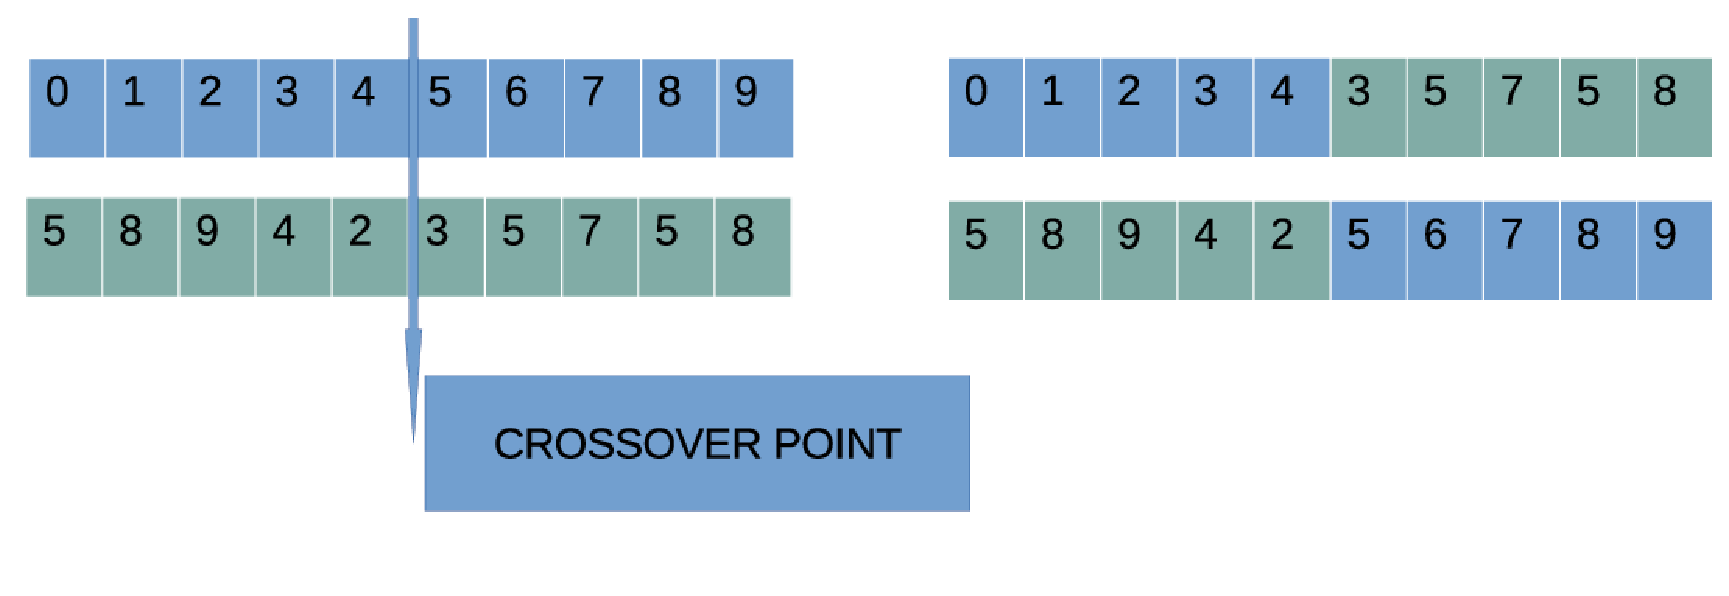
\includegraphics[scale=0.35]{onepoint_crossover}
\par\end{centering}
\caption{An example of the one - point crossover procedure.\protect\label{fig:onePoint}}

\end{figure}


\subsection{Feature construction using Grammatical Evolution \protect\label{subsec:Feature-construction-using}}

The next method used in the performed experiments is the Feature Construction
technique, initially presented in the work of Gavrilis et al \citep{fc1}.
The method utilizes the Grammatical Evolution procedure to create
artificial features from the original ones and hence it can be used
to enhance the effectiveness of any applied machine learning model
to the artificial data. The artificial features are non - linear mappings
of the original ones and the grammar used by the method to construct
such features is shown in Figure \ref{fig:fcGrammar}. 

\begin{figure}[H]
\caption{The grammar used in Feature Construction method.\protect\label{fig:fcGrammar}}

\begin{lyxcode}
S::=\textless expr\textgreater ~~~(0)~

\textless expr\textgreater ~::=~~(\textless expr\textgreater ~\textless op\textgreater ~\textless expr\textgreater )~~~~~~~~~~~~~~~

~~~~~~~~~~~\textbar ~\textless func\textgreater ~(~\textless expr\textgreater ~)~~~~~~~~~~~~~~~~~

~~~~~~~~~~~\textbar\textless terminal\textgreater ~~~~~~~~~~~~~

\textless op\textgreater ~::=~~~~~+~~~~~~~~~~~~~~~~~~~

~~~~~~~~~~~\textbar ~-~~~~~~~~~~~~~~~~~~~

~~~~~~~~~~~\textbar ~{*}~~~~~~~~~~~~~~~~~~~

~~~~~~~~~~~\textbar ~/~~~~~~

\textless func\textgreater ~::=~~~sin~~~~~~~~~~~~~~~

~~~~~~~~~~~\textbar ~cos~~~~~~~~~~~~~~~

~~~~~~~~~~~\textbar exp~~~~~~~~~~~~~~~~

~~~~~~~~~~~\textbar log~~~

\textless terminal\textgreater ::=\textless xlist\textgreater ~~~~~~~~~~~~~~~~~~~~~~~~~~~~~~~~~~~~~~

~~~~~~~~~~~\textbar\textless digitlist\textgreater .\textless digitlist\textgreater ~

\textless xlist\textgreater ::=x1~~~~~~~~~~~~~~~~~~

~~~~~~~~~~~\textbar ~x2~~~~~~~~~~~~~~~

~~~~~~~~~~~………~~~~~~~~~~~~~

~~~~~~~~~~~\textbar ~xN~

\textless digitlist\textgreater ::=\textless digit\textgreater ~~~~~~~~~~~~~~~~~~~~~~~~~~~~~~~~~~~

~~~~~~~~~~~\textbar ~\textless digit\textgreater\textless digit\textgreater ~~~~~~~~~~~~

~~~~~~~~~~~\textbar ~\textless digit\textgreater\textless digit\textgreater\textless digit\textgreater ~~~~~

\textless digit\textgreater ~~::=~0~\textbar ~1~\textbar ~2~\textbar ~3\textbar ~4\textbar ~5\textbar ~6\textbar ~7\textbar ~8\textbar ~9~
\end{lyxcode}
\end{figure}
This method has been incorporated in a series of real - world applications,
such as Spam detection \citep{fc2}, Fetal heart classification \citep{fc3},
classification of EEG signals \citep{fc4,fc5} etc. The features produced
by this procedure can be evaluated using any machine learning method,
although the Radial Basis Function (RBF) networks \citep{rbf1,rbf2}
were used due to the speed of their corresponding training procedure.
The main steps of this procedure are the following:
\begin{enumerate}
\item \textbf{Initialization step}.
\begin{enumerate}
\item \textbf{Define} as $N_{c}$ the number of chromosomes and as $N_{g}$
the number of allowed generations.
\item \textbf{Define} the selection rate $p_{s}$ and the mutation rate
$p_{m}$.
\item \textbf{Define} as $N_{f}$ the number of constructed features.
\item \textbf{Initialize} the $c_{i},\ i=1,\ldots,N_{c}$ chromosomes as
vectors of randomly selected integers.
\item \textbf{Set} $k=0$, the generation counter.
\end{enumerate}
\item \textbf{Fitness calculation step}.
\begin{enumerate}
\item \textbf{For} $i=1,\ldots,N_{c}$ \textbf{do}
\begin{enumerate}
\item \textbf{Create} $N_{f}$ artificial features $y_{1},y_{2},\ldots,y_{N_{f}}$
for the chromosome $c_{i}$. The production is performed using the
grammar of Figure \ref{fig:fcGrammar}.
\item \textbf{Modify} the train set of the objective problem using the features
$y_{1},y_{2},\ldots,y_{N_{f}}$.
\item \textbf{Apply} a machine learning model to the modified set and define
as the fitness value $f_{i}$ the corresponding training error.
\end{enumerate}
\item \textbf{End For}
\end{enumerate}
\item \textbf{Application of genetic operations}. Apply the same genetic
operations as in the case of Neural Construction method of subsection
\ref{subsec:Neural-Network-Construction}.
\item \textbf{Termination check step}.
\begin{enumerate}
\item \textbf{Set} $k=k+1$
\item \textbf{If} $k<N_{g}$ go to Fitness calculation step.
\end{enumerate}
\item \textbf{Testing step}.
\begin{enumerate}
\item \textbf{Obtain} the chromosome $c^{*}$ with the lowest fitness value.
\item \textbf{Produce} the features $y_{1}^{*},y_{2}^{*},\ldots,y_{N_{f}}^{*}$
for this chromosome.
\item \textbf{Modify} the test set of the objective problem using the previously
created features.
\item \textbf{Apply} any machine learning model to the test set and report
the associated error.
\end{enumerate}
\end{enumerate}

\subsection{Create classification rules using Grammatical Evolution\protect\label{subsec:Create-classification-rules}}

The third method used in the conducted experiments which is based
on Grammatical Evolution is the method that produces classification
rules \citep{genclass}. This method has also been published as a
software recently \citep{genclass_softx}. The BNF grammar used by
this method is shown in Figure \ref{fig:genclassGrammar}.

\begin{figure}[H]
\caption{The grammar used by the method that produces classification rules
using Grammatical Evolution.\protect\label{fig:genclassGrammar}}

\begin{lyxcode}
\textless S\textgreater ::=if(\textless BEXPR\textgreater )~CLASS=0~else~CLASS=1~

\textless BEXPR\textgreater ::=\textless XLIST\textgreater\textless BOOLOP\textgreater\textless EXPR\textgreater ~~~~~~~~~~~~

~~~~~~~~~\textbar !(\textless BEXPR\textgreater )~~~~~~~~~~~~~~~~~~~~~~~

~~~~~~~~~\textbar\textless XLIST\textgreater\textless BOOLOP\textgreater\textless EXPR\textgreater\&\textless BEXPR\textgreater ~~~~

~~~~~~~~~\textbar\textless XLIST\textgreater\textless BOOLOP\textgreater\textless EXPR\textgreater\textbar\textless BEXPR\textgreater ~~~~

\textless BOOLOP\textgreater ::=~\textgreater ~~~~~~~~~~~~~~~~~~~~~~~~~~~~~~

~~~~~~~~~~\textbar ~\textgreater =~~~~~~~~~~~~~~~~~~~~~~~~~~~~~

~~~~~~~~~~\textbar ~\textless ~~~~~~~~~~~~~~~~~~~~~~~~~~~~~~

~~~~~~~~~~\textbar ~\textless =~~~~~~~~~~~~~~~~~~~~~~~~~~~~~

\textless EXPR\textgreater ::=~(\textless EXPR\textgreater\textless BINARYOP\textgreater\textless EXPR\textgreater )~~~~~~~~~

~~~~~~~~\textbar ~\textless FUNCTION\textgreater (\textless EXPR\textgreater )~~~~~~~~~~~~~~~

~~~~~~~~\textbar ~\textless TERMINAL\textgreater ~~~~~~~~~~~~~~~~~~~~~~~

\textless BINARYOP\textgreater ::=~+~~~~~~~~~~~~~~~~~~~~~~~~~~~~

~~~~~~~~~~~~\textbar ~-~~~~~~~~~~~~~~~~~~~~~~~~~~~~

~~~~~~~~~~~~\textbar ~{*}~~~~~~~~~~~~~~~~~~~~~~~~~~~~

~~~~~~~~~~~~\textbar ~/~~~~~~~~~~~~~~~~~~~~~~~~~~~~

\textless FUNCTION\textgreater ::=~sin~\textbar ~cos~\textbar ~exp~\textbar ~log~~~~~~~~

\textless TERMINAL\textgreater ::=~\textless XLIST\textgreater ~~~~~~~~~~~~~~~~~~~~~~

~~~~~~~~~~~~\textbar ~\textless DIGITLIST\textgreater .\textless DIGITLIST\textgreater ~~~~~~

~~~~~~~~~~~~\textbar ~(-\textless DIGITLIST\textgreater .\textless DIGITLIST\textgreater )~~~

~\textless XLIST\textgreater ::=~x1~\textbar ~x2~\textbar ~...\textbar xD~~~~~~~~~~~~~~~

\textless DIGITLIST\textgreater ::=\textless DIGIT\textgreater ~~~~~~~~~~~~~~~~~~~~~~

~~~~~~~~~~~~~\textbar ~\textless DIGIT\textgreater\textless DIGIT\textgreater ~~~~~~~~~~~~~~

~~~~~~~~~~~~~\textbar ~\textless DIGIT\textgreater\textless DIGIT\textgreater\textless DIGIT\textgreater ~~~~~~~

\textless DIGIT\textgreater ::=~0~\textbar ~1~\textbar ~2~\textbar ~3~\textbar ~4~\textbar 5~\textbar 6~\textbar 7~\textbar 8~\textbar 9~~~~
\end{lyxcode}
\end{figure}
The main steps of this method have as follows:
\begin{enumerate}
\item \textbf{Initialization step}.
\begin{enumerate}
\item \textbf{Define} as $N_{c}$ the total number of chromosomes and with
$N_{g}$ the allowed number of generations.
\item \textbf{Define} the selection rate $p_{s}$ and the mutation rate
$p_{m}$.
\item \textbf{Initialize} as vectors of randomly selected integers the chromosomes
$c_{i},\ i=1,\ldots,N_{c}$.
\item \textbf{Set} $k=0$, the generation counter.
\end{enumerate}
\item \textbf{Fitness calculation step}.
\begin{enumerate}
\item \textbf{For} $i=1,\ldots,N_{c}$ \textbf{do} 
\begin{enumerate}
\item \textbf{Create} using the Grammatical evolution procedure and the
grammar depicted in Figure \ref{fig:genclassGrammar} a classification
program $G_{i}$ for the corresponding chromosome $c_{i}$. 
\item \textbf{Set} the fitness $f_{i}$ as
\begin{equation}
f_{i}=\sum_{j=1}^{M}\left(G_{i}\left(x_{j}\right)-t_{j}\right)^{2}
\end{equation}
for the corresponding training set $T=\left\{ \left(x_{1},t_{1}\right),\left(x_{2},t_{2}\right),\ldots,\left(x_{M},t_{M}\right)\right\} $.
The values $x_{i}$ denote the input patterns and the value $t_{i}$
the expected outcome for pattern $x_{i}$.
\end{enumerate}
\item \textbf{End For}
\end{enumerate}
\item \textbf{Genetic operations step}. Apply the same genetic operations
as in the case of Neural Construction method of subsection \ref{subsec:Neural-Network-Construction}.
\item \textbf{Termination check step}.
\begin{enumerate}
\item \textbf{Set} $k=k+1$
\item \textbf{If} $k<N_{g}$ then go to Fitness calculation step.
\end{enumerate}
\item \textbf{Testing step}.
\begin{enumerate}
\item \textbf{Obtain} the best chromosome $c^{*}$ and produce the associated
classification program $G^{*}$.
\item \textbf{Apply} the classification program to the test set of the problem
and report the result.
\end{enumerate}
\end{enumerate}

\section{Results\protect\label{sec:Results}}

The code used in the experiments was implemented in C++ programming
language with the assistance of Optimus optimization environment,
freely available from \url{https://github.com/itsoulos/GlobalOptimus/}
(accessed on 2 April 2025). Also, the freely available programming
tool of WEKA \citep{weka_main} was used for some of the experiments,
that can be downloaded also freely from \url{https://ml.cms.waikato.ac.nz/weka/}(accessed
on 2 April 2025). For the validation of the experiments the method
of ten - fold cross validation was incorporated. All the experiments
were conducted on a machine running Debian Linux with 128GB of RAM.
The values for the experimental settings are shown in Table \ref{tab:settings}.

\begin{table}[H]
\caption{The values used for the experimental settings.\protect\label{tab:settings}}

\centering{}%
\begin{tabular}{|c|c|c|}
\hline 
PARAMETER & MEANING & VALUE\tabularnewline
\hline 
\hline 
$N_{c}$ & Number of chromosomes & 500\tabularnewline
\hline 
$N_{g}$ & Maximum number of generations & 200\tabularnewline
\hline 
$p_{s}$ & Selection rate & 0.10\tabularnewline
\hline 
$p_{m}$ & Mutation rate & 0.05\tabularnewline
\hline 
$N_{f}$ & Number of produced features & 2\tabularnewline
\hline 
$H$  & Number or processing nodes & 10\tabularnewline
\hline 
\end{tabular}
\end{table}
Also, the Table \ref{tab:exper} contains the experimental results
where the following notation is used:
\begin{enumerate}
\item The column YEAR denotes denotes the year for which the methods were
applied. 
\item The column BAYES NET denotes the application of the Bayesian Network
method \citep{bayes_net1,bayes_net2}.
\item The column MLP represents the incorporation of an artificial neural
network with $H=10$ processing nodes, that was trained using the
Back Propagation method \citep{bpnn1,bpnn2}.
\item The column RBF denotes the usage of a Radial Basis Function network
with $H=10$ processing nodes.
\item The column NNC represents the usage of the Neural Network construction
method described in subsection \ref{subsec:Neural-Network-Construction}.
\item The column FC stands for the usage of the Feature Construction method
provided in subsection \ref{subsec:Feature-construction-using}.
\item The column GENCLASS denotes the usage of the method that creates classification
rules, described in subsection \ref{subsec:Create-classification-rules}.
\item The final row AVERAGE represents the average classification error
for all years between 2014 and 2023.
\end{enumerate}
\begin{table}[H]
\caption{Experimental results using various machine learning techniques. Numbers
in cells represent average classification error as measured on the
corresponding test set. \protect\label{tab:exper}}

\centering{}%
\begin{tabular}{|c|c|c|c|c|c|c|}
\hline 
\textbf{YEAR} & \textbf{BAYES NET} & \textbf{MLP} & \textbf{RBF} & \textbf{NNC} & \textbf{FC} & \textbf{GENCLASS}\tabularnewline
\hline 
\hline 
2014 & 9.01\% & 8.34\% & 11.97\% & 7.82\% & 7.35\% & 7.03\%\tabularnewline
\hline 
2015 & 8.75\% & 7.63\% & 10.79\% & 7.13\% & 6.78\% & 6.65\%\tabularnewline
\hline 
2016 & 8.99\% & 8.13\% & 10.73\% & 7.48\% & 7.10\% & 7.05\%\tabularnewline
\hline 
2017 & 8.43\% & 8.29\% & 10.78\% & 7.68\% & 7.24\% & 7.13\%\tabularnewline
\hline 
2018 & 8.38\% & 7.99\% & 9.33\% & 7.30\% & 7.11\% & 6.74\%\tabularnewline
\hline 
2019 & 7.31\% & 7.78\% & 24.81\% & 7.33\% & 7.15\% & 6.26\%\tabularnewline
\hline 
2020 & 8.70\% & 7.86\% & 10.03\% & 6.99\% & 6.66\% & 6.47\%\tabularnewline
\hline 
2021 & 8.58\% & 7.88\% & 10.37\% & 6.87\% & 6.55\% & 6.39\%\tabularnewline
\hline 
2022 & 8.80\% & 7.29\% & 8.45\% & 6.86\% & 6.52\% & 6.32\%\tabularnewline
\hline 
2023 & 8.46\% & 7.50\% & 10.56\% & 6.87\% & 6.58\% & 6.20\%\tabularnewline
\hline 
\textbf{AVERAGE} & \textbf{8.54\%} & \textbf{7.87\%} & \textbf{11.78\%} & \textbf{7.23\%} & \textbf{6.90\%} & \textbf{6.62\%}\tabularnewline
\hline 
\end{tabular}
\end{table}
In Table \ref{tab:exper} GENCLASS demonstrates the lowest average
classification error (6.62\%), making it the most reliable model for
wildfire prediction. It is followed by FC with an average error of
6.90\% and NNC with 7.23\%. Traditional models such as BAYES NET (8.54\%)
and MLP(BP) (7.87\%) exhibit higher error rates, while RBF performs
the worst with an average error of 11.78\%, including an exceptionally
high value in 2019 (24.81\%), likely due to overfitting or sensitivity
to outliers. GENCLASS not only has the lowest error but also shows
consistent improvement over time. Starting at 7.03\% in 2014, it decreased
to 6.20\% in 2023, with minor fluctuations in between. FC and NNC
also display a declining trend but with greater variability. In contrast,
MLP(BP) and BAYES NET show no clear improvement, with BAYES NET even
experiencing a slight increase in error in 2022--2023. RBF, despite
improving after 2019, remains unstable and less reliable. When comparing
the top three models (GENCLASS, FC, NNC), GENCLASS consistently outperforms
the others in all years except 2019, where FC had a marginally better
performance. NNC, while superior to traditional methods, lags behind
GENCLASS and FC. The remaining models (BAYES NET, MLP(BP), RBF) appear
less competitive in accuracy compared to newer techniques. The data
strongly supports GENCLASS as the optimal model for wildfire prediction
due to its consistently low and stable error rate, as well as its
progressive improvement over time. FC and NNC remain viable alternatives
with good performance, but GENCLASS maintains a clear advantage. The
other models, particularly RBF, may require further optimization to
enhance reliability. The steady performance of GENCLASS makes it the
safest choice for practical applications.

Within the framework of statistical analysis, R language scripts were
executed to extract significance levels (p-values) for performance
differences between the classification models. The results, shown
in Figure \ref{fig:stat}, reveal statistically significant differences
between the compared models. Specifically, all pairwise model comparisons
yielded p-values below the standard significance threshold (typically
p \textless{} 0.05), indicating statistically significant performance
differences. The comparison between BAYES NET and MLP(BP) produced
p = 0.0098, while BAYES NET's comparisons with RBF, NNC, FC and GENCLASS
showed even smaller values (p = 0.0039 and p = 0.002), confirming
that BAYES NET differs significantly from other models. Similarly,
MLP(BP) comparisons with RBF, NNC, FC and GENCLASS all resulted in
p = 0.002, demonstrating high statistical significance in their performance
differences. The same holds true for RBF's comparisons with NNC, FC
and GENCLASS (p = 0.002), as well as for comparisons between NNC,
FC and GENCLASS. The fact that all p-values are very small (p \ensuremath{\le}
0.0098) confirms that the models do not perform equally and that statistically
significant differences exist between them. This is particularly evident
in comparisons involving GENCLASS, which - as previous analysis has
shown - stands out for its high accuracy. These results reinforce
the conclusion that certain models (such as GENCLASS and FC) are clearly
superior to others (like BAYES NET and RBF), a finding that should
be considered in practical machine learning applications.

\begin{figure}
\begin{centering}
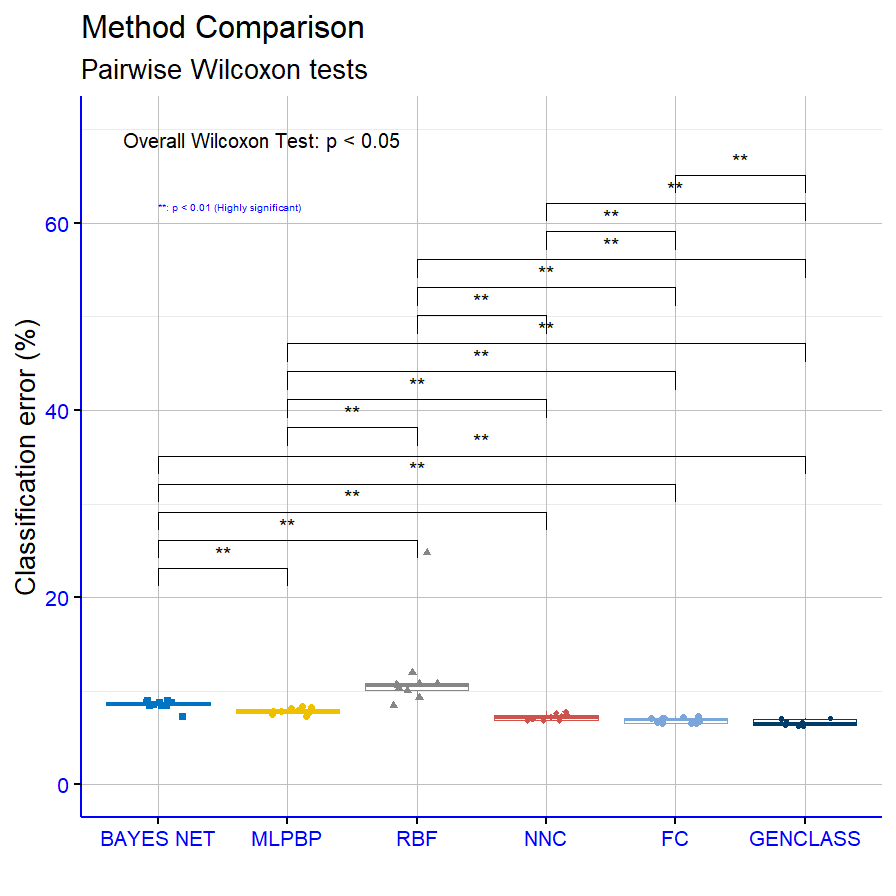
\includegraphics[scale=0.5]{stat}
\par\end{centering}
\caption{Statistical comparison of the experimental results obtained by various
machine learning methods.\protect\label{fig:stat}}

\end{figure}


\section{Conclusions\protect\label{sec:Conclusions}}

This study implements the innovative technique of Grammatical Evolution
to predict the consequences of urban fires, utilizing a decade of
data from the Hellenic Fire Service. The results demonstrate the clear
superiority of the GENCLASS method over other machine learning approaches,
both in terms of accuracy and interpretability. The method's ability
to generate human-readable classification rules constitutes a significant
advantage over traditional \textquotedbl black-box\textquotedbl{}
machine learning models. These rules reveal complex correlations between
factors such as meteorological conditions, urban layout, and human
activity, providing valuable insights for fire prevention and management.
However, the research does face certain limitations that warrant discussion.
The reliance on historical data reduces predictive capability in extreme
or unprecedented scenarios, such as those caused by climate change.
Additionally, the performance of some models, like RBF, shows significant
instability in certain cases, likely due to overfitting or sensitivity
to outliers. This underscores the need for further algorithm optimization
and the integration of additional data to enhance reliability.

The findings of this research confirm that Grammatical Evolution,
particularly the GENCLASS method, offers a robust solution for predicting
the impacts of urban fires. This method not only achieves the lowest
average classification error but also provides transparent, interpretable
rules that can be directly utilized by fire departments and urban
planners. The generated rules uncover critical dependencies, such
as the influence of temperature, emergency response times, and demographic
characteristics on the extent of damage. This paves the way for developing
dynamic evacuation strategies, implementing preventive measures in
vulnerable areas, and raising public awareness of fire risks. Moreover,
the consistent improvement in GENCLASS's performance over time suggests
its adaptability to changing conditions and its potential for enhancement
with new data. However, it is important to recognize that the effectiveness
of any predictive method depends heavily on the quality and completeness
of available data, as well as the ability to account for new and unforeseen
factors, such as climate change.

To further develop the findings of this research and strengthen their
practical application, several directions for future exploration are
proposed. First, the integration of real-time data from sensors and
satellite systems could significantly improve the accuracy and timeliness
of predictions, enabling dynamic model adjustments and rapid responses
to emerging threats. Second, extending the method to other geographic
regions with different urban and climatic characteristics could explore
the generalizability of the findings and identify new factors influencing
fire risk. Third, combining Grammatical Evolution with advanced deep
learning techniques, such as neural networks for spatiotemporal analysis,
could enhance predictive capabilities in complex scenarios involving
multiple simultaneous hazards. Finally, developing simulations that
account for the long-term impacts of climate change and urban expansion
could provide valuable insights for designing more resilient and safer
urban environments. These directions have the potential to transform
the research findings into practical tools for safeguarding human
lives and urban infrastructure.

\vspace{6pt}


\authorcontributions{C.K., V.C. and I.G.T. conceived of the idea and the methodology,
and C.K. and V.C. implemented the corresponding software. C.K. conducted
the experiments, employing objective functions as test cases, and
provided the comparative experiments. A.M. performed the necessary
statistical tests. All authors have read and agreed to the published
version of the manuscript.}

\funding{This research received no external funding.}

\institutionalreview{Not applicable.}

\informedconsent{Not applicable.}

\acknowledgments{This research has been financed by the European Union : Next Generation
EU through the Program Greece 2.0 National Recovery and Resilience
Plan , under the call RESEARCH -- CREATE -- INNOVATE, project name
“iCREW: Intelligent small craft simulator for advanced crew training
using Virtual Reality techniques\textquotedbl{} (project code:TAEDK-06195).
\quad{}}

\conflictsofinterest{The authors declare no conflicts of interest.}

\appendix

\begin{adjustwidth}{-\extralength}{0cm}{}

\reftitle{References}
\begin{thebibliography}{999}
\bibitem[Author1(year)]{fire_ref1}Fires -- Wildfires and Urban Fires.
Juniata County Appendix CMulti-Jurisdictional Hazard Mitigation Plan
Hazard Profiles. 2008. Pp. 15-19. Available from: \url{https://juniataco.org/docs/hmp/Appendix%20C%20-%2004-Fire-Urban%20and%20Rural.pdf }
(Accessed on 07 March 2025 ).

\bibitem[(year)]{fire_ref2}M.R. Hossain, O. Smirnov, Analyzing the
risk factors of residential fires in urban and rural census tracts
of Ohio using panel data analysis, Applied geography \textbf{151},
102863, 2023.

\bibitem[Author2(year)]{hellenic_fire} Hellenic Fire Service. Open
Data. Incident record. Available from: \url{https://www.fireservice.gr/el_GR/synola-dedomenon}
(Accessed on 07 March 2025 ).

\bibitem[(year)]{greek_wikipedia}Greek Wikipedia. The trial regarding
MATI's wildfire. Available from: \url{https://el.wikipedia.org/wiki/%CE%94%CE%AF%CE%BA%CE%B7_%CE%B3%CE%B9%CE%B1_%CF%84%CE%BF_%CE%9C%CE%AC%CF%84%CE%B9}
(Accessed on 27 February 2025).

\bibitem[(year)]{greek_wildfire}G. Xanthopoulos, M. Athanasiou, Uniting
Our Global Wildfire Community. Wildfire, International Association
of Wildland Fire. April 2019, volume 28.2. 

\bibitem[(year)]{who}World Health Organization (WHO). Burns. 13 October
2023. Available from: \url{https://www.who.int/news-room/fact-sheets/detail/burns}
(Accessed on 13 March 2025).

\bibitem[(year)]{fire_hazards}Natural Hazards Research Australia.
Understanding the Black Summer bushfires through research: a summary
of key finding from the Bushfire and Natural Hazards CRC. January
2023. Available from: \url{https://www.naturalhazards.com.au/sites/default/files/2023-01/Understanding%20the%20Black%20Summer%20bushfires%20through%20research_final_web_NHRA.pdf}
(Accessed on 13 March 2025).

\bibitem[(year)]{australian_report}Australian Government. Australian
Public Service Commission. Black Summer. State of the Service Report
2019 -- 20. Available from: \url{https://www.apsc.gov.au/state-service/state-service-report-2019-20/chapter-1-commitment-service/black-summer}
(Accessed on 13 March 2025).

\bibitem[(year)]{fires_siberian}Fires char the Siberian Arctic. NASA,
Earth observatory. 10 July 2024. Available from:\url{ https://earthobservatory.nasa.gov/images/153087/fires-char-the-siberian-arctic}
(Accessed on 17 March 2025).

\bibitem[(year)]{nasa_images}Landsat Image Gallery. NASA. Available
from: \url{https://landsat.visibleearth.nasa.gov/view.php?id=153087 }
(Accessed on 17 March 2025) . 

\bibitem[(year)]{fires_russia}Raging Wildfires Devastate Russia’s
Far East Sakha Republic. The Moscow Times. By Leyla Latypova. 23 July
2024. Available from: \url{https://www.themoscowtimes.com/2024/07/23/raging-wildfires-devastate-russias-far-east-sakha-republic-a85802}
(Accessed on 17 March 2025) .

\bibitem[(year)]{fire_cities}Cities face rising fire risks from climate
change without emission cuts. ChosunBiz. By Park Keun-tae. 03 March
2025. Available from: \url{https://biz.chosun.com/en/en-science/2025/03/05/FXRLKFRXJJB5LK4YXKPLVETVJM/}
( Accessed on 17 March 2025) . 

\bibitem[(year)]{fire_climate}Here’s how climate change fueled the
Los Angeles fires. Npr org. By Lauren Sommer. 29 January 2025. Available
from: \url{https://www.npr.org/2025/01/29/nx-s1-5273676/la-fires-climate-change-rainfall-extreme-weather }
(Accessed on 17 March 2025 ). 

\bibitem[(year)]{fire_graphics}Graphics Explain Los Angeles ‘ Rare
and Devastating January Fires. World Resources Institute. Wri org.
By James McCarthy \& Jessica Richter. 05 February 2025. Available
from: \url{https://www.wri.org/insights/los-angeles-fires-january-2025-explained}
( Accessed on 17 March 2025 ).

\bibitem[(year)]{fire_japan}Fire Grows Unusually Large in Japan.
NASA. Earth observatory. Available from: \url{https://earthobservatory.nasa.gov/images/154008/fire-grows-unusually-large-in-japan}
( Accessed on 17 March 2025 ). 

\bibitem[(year)]{fire_bbc}Thousands evacuated as Japan’s biggest
fire in decades continues to burn. BBC. By Gavin Butler. 03 March
17, 2025. Available from: \url{https://www.bbc.com/news/articles/c89ypkq72d0o}
(Accessed on 17 March 2025 ). 

\bibitem[(year)]{fire_turkey}E. Ceyhan, K. Ertugay, S. Duzgun, Exploratory
and inferential methods for spatio-temporal analysis of residential
fire clustering in urban areas, Fire safety Journal \textbf{58}, pp.
226-239, 2013.

\bibitem[(year)]{fire_social}C.R. Jennings, Social and economic characteristics
as determinants of residential fire risk in urban neighborhoods: A
review of the literature, Fire safety Journal \textbf{62}, pp. 13-19,
2013.

\bibitem[(year)]{fire_resident}D. Rohde, J. Corcoran, P. Chhetri,
Spatial forecasting of residential urban fires: A Bayesian approach.
Computers, Environment and Urban Systems \textbf{34}, pp. 58-69, 2010.

\bibitem[(year)]{fire_model}R. Ardianto, P. Chhetri, Modeling Spatial-Temporal
Dynamic of Urban Residential Fire Risk Using a Markov Chain Technique,
International Journal of Disaster Risk Science \textbf{10}, pp. 57-73,
2019. 

\bibitem[(year)]{fire_freq}J. Clare, L. Garis, D. Plecas, C. Jennings,
Reduced frequency and severity of residential fires following delivery
of fire prevention education by on-duty fire fighters: Cluster randomized
controlled study, Journal of Safety Research \textbf{43}, pp. 123-128,
2012.

\bibitem[(year)]{fire_risk_manage}S. Alkis, E. Aksoy, K. Akpinar,
Risk Assessment of Industrial Fires for Surrounding Vulnerable Facilities
Using a Multi- Criteria Decision Support Approach and GIS, Fire \textbf{ 4},
53, 2021.

\bibitem[(year)]{fire_gis}Y. Jiang, A. Lv, Z. Yan, Z. Yang, A GIS-Based
Multi-Criterion Decision-Making Method to Select City Fire Brigade:
A Case Study of Wuhan, China, International Journal of Geo-Information.
ISPRS \textbf{10}, 777, 2021. 

\bibitem[(2020)]{svm}Suthaharan, S., \& Suthaharan, S. (2016). Support
vector machine. Machine learning models and algorithms for big data
classification: thinking with examples for effective learning, 207-235.

\bibitem[(year)]{fire_prob}Y. Maniatis, A. Doganis, M. Chatzigeorgiadis,
Fire Risk Probability Mapping Using Machine Learning Tools and Multi
-- Criteria Decision Analysis in the GIS Environment: A Case Study
in the National Park Forest Dadia-Lefkimi-Soufli, Greece, Applied
Science \textbf{12}, 2938, 2022.

\bibitem[(year)]{fire_gis_model}S. Noori, A. Mohammadi, T. Ferreira,
G. Miguel., A. Gilandeh, M. Ghaffari, S. Ardabili, J. Seyed, Modelling
and Mapping Urban Vulnerability Index against Potential Structural
Fire-related Risks: An Integrated GIS-MCDM Approach, Fire \textbf{6},
107, 2023.

\bibitem[(year)]{fire_big_data}C-A. Lee, Y.-C. Sung, Y-S. Lin, G.K-K.
Hsiao, Evaluating the severity of building fires with the analytical
hierarchy process, big data analysis, and remote sensing, Natural
Hazards \textbf{103}, pp. 1843-1856, 2020.

\bibitem[(2020)]{fire_safety}C.-A. Lee, Y-C. Sung, , Y-S. Lin, G.
K-K. Hsiao, Evaluating the severity of building fires with the analytical
hierarchy process, big data analysis, and remote sensing, Natural
Hazards \textbf{103},pp. 1843-1856, 2020.

\bibitem[(2020)]{random_forest1}L. Breiman, Random forests, Machine
learning \textbf{45}, pp. 5-32, 2001.

\bibitem{random_forest2}S.J. Rigatti, Random forest, Journal of Insurance
Medicine \textbf{47}, pp. 31-39, 2017.

\bibitem[(2020)]{xgboost}Chen, T., \& Guestrin, C. (2016, August).
Xgboost: A scalable tree boosting system. In Proceedings of the 22nd
acm sigkdd international conference on knowledge discovery and data
mining (pp. 785-794).

\bibitem[(2020)]{fire_station}Dey, Arnab., Heger, Andrew., England,
Darin. Urban Fire Station Planning using Predicted Demand and Service
Quality Index. Springer Nature 2021. 

\bibitem[(2020)]{bwm}Pamučar, D., Ecer, F., Cirovic, G., \& Arlasheedi,
M. A. (2020). Application of improved best worst method (BWM) in real-world
problems. Mathematics, 8(8), 1342.

\bibitem[(2020)]{mcdm}Taherdoost, H., \& Madanchian, M. (2023). Multi-criteria
decision making (MCDM) methods and concepts. Encyclopedia, 3(1), 77-87.

\bibitem[(2020)]{fire_decision_maker}Erden, Turan., Hopkins Nyimbili,
Penjani. Comparative evaluation of GIS-based best -- worst method
(BMW) for emergency facility planning: perspectives from two decision-maker
groups. Natural Hazards, volume 105, issue 1. January 2021. Pp. 1031-1067.

\bibitem[(2020)]{fire_risk_prediction}Singh Walia, Bhavkaran., Hu,
Qiany., Chen, Jeffrey., Chen, Fangyan., Lee, Jessica., et al. A Dynamic
pipeline for Spatio -Temporal Fire Risk Prediction. Proceedings of
the 24th ACM SIGKDD International Conference on Knowledge Discovery
\& Data Mining.2018. pp. 764--773. 

\bibitem[(2020)]{fire_forecast}G. Jin, Q. Wang, C. Zhu, Y. Feng,
J. Huang, X. Hu, Urban Fire Situation Forecasting: Deep sequence learning
with Spatio -- temporal dynamics, Applied Soft Computing \textbf{97},
2020. 

\bibitem[(2020)]{kmeans}MacQueen, J.: Some methods for classification
and analysis of multivariate observations, in: Proceedings of the
fifth Berkeley symposium on mathematical statistics and probability,
Vol. 1, No. 14, pp. 281-297, 1967. 

\bibitem[(2020)]{fire_stat}W. Lizhi, R. Aizhu, Urban Fire Risk Clustering
Method Based on Fire Statistics, Tsinghua science \& Technology \textbf{13},
pp. 418 -- 422, 2008.

\bibitem[(2020)]{fire_nepal}K. KC, R. Ardianto, P. Chhetri, J. Corcoran,
Geographic patterns of urban fires in the global south: the case of
Kathmandu, Nepal. GeoJournal \textbf{89}, 137, 2024.

\bibitem[(2020)]{fire_ml}A. Sahebi, B. Havasy, Y. Veisani, Predicting
firefighting operation time in urban areas using machine learning:
identifying key determinants for improved emergency response, Discover
Applied Science \textbf{7}, 2025.

\bibitem[(2020)]{fire_deep}A.A. Ishola, D. Valles, Enhancing safety
and Efficiency in Firefighting Operations via Deep Learning and Temperature
Forecasting Modeling in Autonomous Unit., Sensors \textbf{ 23}, 4628,
2023.

\bibitem[(2020)]{fire_time_series}T. Nishino, A. Hokugo, A stochastic
model for time series prediction of the number of post -- earthquake
fire ignition in buildings based on the ignition record for the 2011
Tohoku Earthquake, Earthquake Spectra \textbf{36}, 2019. 

\bibitem[(2020)]{fire_simulation}T. Nishino, Physics -- based urban
fires spread simulation coupled with stochastic occurrence of spot
fires, Stochastic Environmental Research and Risk Assessment \textbf{33},
pp. 451 -- 463, 2019.

\bibitem[(2020)]{fire_earthquake}T. Nishino, Probabilistic urban
cascading multi-hazard risk assessment methodology for ground shaking
and post -- earthquake fires, Natural Hazards \textbf{116}, pp. 3165
-- 3200, 2023.

\bibitem{ge1}M. O’Neill, C. Ryan, Grammatical evolution, IEEE Trans.
Evol. Comput. \textbf{5,}pp. 349--358, 2001.

\bibitem[(2020)]{nn1}C. Bishop, Neural Networks for Pattern Recognition,
Oxford University Press, 1995.

\bibitem{nn2}G. Cybenko, Approximation by superpositions of a sigmoidal
function, Mathematics of Control Signals and Systems \textbf{2}, pp.
303-314, 1989.

\bibitem[(year)]{bnf1}J. W. Backus. The Syntax and Semantics of the
Proposed International Algebraic Language of the Zurich ACM-GAMM Conference.
Proceedings of the International Conference on Information Processing,
UNESCO, 1959, pp.125-132.

\bibitem{ge_program1}C. Ryan, J. Collins, M. O’Neill, Grammatical
evolution: Evolving programs for an arbitrary language. In: Banzhaf,
W., Poli, R., Schoenauer, M., Fogarty, T.C. (eds) Genetic Programming.
EuroGP 1998. Lecture Notes in Computer Science, vol 1391. Springer,
Berlin, Heidelberg, 1998.

\bibitem{ge_program2}M. O’Neill, M., C. Ryan, Evolving Multi-line
Compilable C Programs. In: Poli, R., Nordin, P., Langdon, W.B., Fogarty,
T.C. (eds) Genetic Programming. EuroGP 1999. Lecture Notes in Computer
Science, vol 1598. Springer, Berlin, Heidelberg, 1999.

\bibitem{ge_trig}C. Ryan, M. O’Neill, J.J. Collins, Grammatical evolution:
Solving trigonometric identities, proceedings of Mendel. Vol. 98.
1998.

\bibitem{ge_music}A.O. Puente, R. S. Alfonso, M. A. Moreno, Automatic
composition of music by means of grammatical evolution, In: APL '02:
Proceedings of the 2002 conference on APL: array processing languages:
lore, problems, and applications July 2002 Pages 148--155. 

\bibitem{ge_nn}Lídio Mauro Limade Campo, R. Célio Limã Oliveira,Mauro
Roisenberg, Optimization of neural networks through grammatical evolution
and a genetic algorithm, Expert Systems with Applications \textbf{56},
pp. 368-384, 2016.

\bibitem{ge_nn2}K. Soltanian, A. Ebnenasir, M. Afsharchi, Modular
Grammatical Evolution for the Generation of Artificial Neural Networks,
Evolutionary Computation \textbf{30}, pp 291--327, 2022.

\bibitem{ge_constant}I. Dempsey, M.O' Neill, A. Brabazon, Constant
creation in grammatical evolution, International Journal of Innovative
Computing and Applications \textbf{1} , pp 23--38, 2007.

\bibitem{ge_pacman}E. Galván-López, J.M. Swafford, M. O’Neill, A.
Brabazon, Evolving a Ms. PacMan Controller Using Grammatical Evolution.
In: , et al. Applications of Evolutionary Computation. EvoApplications
2010. Lecture Notes in Computer Science, vol 6024. Springer, Berlin,
Heidelberg, 2010.

\bibitem{ge_supermario}N. Shaker, M. Nicolau, G. N. Yannakakis, J.
Togelius, M. O'Neill, Evolving levels for Super Mario Bros using grammatical
evolution, 2012 IEEE Conference on Computational Intelligence and
Games (CIG), 2012, pp. 304-31.

\bibitem{ge_energy}D. Martínez-Rodríguez, J. M. Colmenar, J. I. Hidalgo,
R.J. Villanueva Micó, S. Salcedo-Sanz, Particle swarm grammatical
evolution for energy demand estimation, Energy Science and Engineering
\textbf{8}, pp. 1068-1079, 2020.

\bibitem{ge_comb}N. R. Sabar, M. Ayob, G. Kendall, R. Qu, Grammatical
Evolution Hyper-Heuristic for Combinatorial Optimization Problems,
IEEE Transactions on Evolutionary Computation \textbf{17}, pp. 840-861,
2013.

\bibitem{ge_crypt}C. Ryan, M. Kshirsagar, G. Vaidya, G. et al. Design
of a cryptographically secure pseudo random number generator with
grammatical evolution. Sci Rep \textbf{12}, 8602, 2022.

\bibitem[(2008)]{nnc}I.G. Tsoulos, D. Gavrilis, E. Glavas, Neural
network construction and training using grammatical evolution, Neurocomputing
\textbf{72}, pp. 269-277, 2008.

\bibitem[(2008)]{nn_amide1}G.V. Papamokos, I.G. Tsoulos, I.N. Demetropoulos,
E. Glavas, Location of amide I mode of vibration in computed data
utilizing constructed neural networks, Expert Systems with Applications
\textbf{36}, pp. 12210-12213, 2009.

\bibitem{nnc_de}I.G. Tsoulos, D. Gavrilis, E. Glavas, Solving differential
equations with constructed neural networks, Neurocomputing \textbf{72},
pp. 2385-2391, 2009.

\bibitem{nnc_feas}I.G. Tsoulos, G. Mitsi, A. Stavrakoudis, S. Papapetropoulos,
Application of Machine Learning in a Parkinson's Disease Digital Biomarker
Dataset Using Neural Network Construction (NNC) Methodology Discriminates
Patient Motor Status, Frontiers in ICT 6, 10, 2019.

\bibitem{nnc_student}V. Christou, I.G. Tsoulos, V. Loupas, A.T. Tzallas,
C. Gogos, P.S. Karvelis, N. Antoniadis, E. Glavas, N. Giannakeas,
Performance and early drop prediction for higher education students
using machine learning, Expert Systems with Applications \textbf{225},
120079, 2023.

\bibitem{nnc_autism}E.I. Toki, J. Pange, G. Tatsis, K. Plachouras,
I.G. Tsoulos, Utilizing Constructed Neural Networks for Autism Screening,
Applied Sciences \textbf{14}, 3053, 2024.

\bibitem[(2008)]{fc1}Dimitris Gavrilis, Ioannis G. Tsoulos, Evangelos
Dermatas, Selecting and constructing features using grammatical evolution,
Pattern Recognition Letters \textbf{29},pp. 1358-1365, 2008. 

\bibitem[(2008)]{fc2}Dimitris Gavrilis, Ioannis G. Tsoulos, Evangelos
Dermatas, Neural Recognition and Genetic Features Selection for Robust
Detection of E-Mail Spam, Advances in Artificial Intelligence Volume
3955 of the series Lecture Notes in Computer Science pp 498-501, 2006.

\bibitem{fc3}George Georgoulas, Dimitris Gavrilis, Ioannis G. Tsoulos,
Chrysostomos Stylios, João Bernardes, Peter P. Groumpos, Novel approach
for fetal heart rate classification introducing grammatical evolution,
Biomedical Signal Processing and Control \textbf{2},pp. 69-79, 2007 

\bibitem{fc4}Otis Smart, Ioannis G. Tsoulos, Dimitris Gavrilis, George
Georgoulas, Grammatical evolution for features of epileptic oscillations
in clinical intracranial electroencephalograms, Expert Systems with
Applications \textbf{38}, pp. 9991-9999, 2011 

\bibitem{fc5}A. T. Tzallas, I. Tsoulos, M. G. Tsipouras, N. Giannakeas,
I. Androulidakis and E. Zaitseva, Classification of EEG signals using
feature creation produced by grammatical evolution, In: 24th Telecommunications
Forum (TELFOR), pp. 1-4, 2016.

\bibitem[(2008)]{rbf1}J. Park and I. W. Sandberg, Universal Approximation
Using Radial-Basis-Function Networks, Neural Computation 3, pp. 246-257,
1991.

\bibitem{rbf2}H. Yu, T. Xie, S. Paszczynski, B. M. Wilamowski, Advantages
of Radial Basis Function Networks for Dynamic System Design, in IEEE
Transactions on Industrial Electronics \textbf{58}, pp. 5438-5450,
2011.

\bibitem[(2008)]{genclass}Tsoulos, I.G. Creating classification rules
using grammatical evolution. Int. J. Comput. Intell. Stud. 2020, 9,
161--171.

\bibitem[(2008)]{genclass_softx}Anastasopoulos, N.; Tsoulos, I.G.;
Tzallas, A. GenClass: A parallel tool for data classification based
on Grammatical Evolution. SoftwareX 2021, 16, 100830.

\bibitem[(2009)]{weka_main}M. Hall, F. Frank, G. Holmes, B. Pfahringer,
P. Reutemann, I.H. Witten, The WEKA data mining software: an update.
ACM SIGKDD explorations newsletter \textbf{11}, pp. 10-18, 2009.

\bibitem[(2009)]{bayes_net1}Ben-Gal, I. (2008). Bayesian Networks.
In Encyclopedia of Statistics in Quality and Reliability (eds F. Ruggeri,
R.S. Kenett and F.W. Faltin).

\bibitem{bayes_net2} Koski, T., \& Noble, J. (2011). Bayesian networks:
an introduction. John Wiley \& Sons.

\bibitem[(2009)]{bpnn1}D.E. Rumelhart, G.E. Hinton and R.J. Williams,
Learning representations by back-propagating errors, Nature \textbf{323},
pp. 533 - 536 , 1986.

\bibitem{bpnn2}T. Chen and S. Zhong, Privacy-Preserving Backpropagation
Neural Network Learning, IEEE Transactions on Neural Networks \textbf{20},
, pp. 1554-1564, 2009.

\end{thebibliography}
%%%%%%%%%%%%%%%%%%%%%%%%%%%%%%%%%%%%%%%%%%
%% for journal Sci
%\reviewreports{\\
%Reviewer 1 comments and authors' response\\
%Reviewer 2 comments and authors' response\\
%Reviewer 3 comments and authors' response
%}
%%%%%%%%%%%%%%%%%%%%%%%%%%%%%%%%%%%%%%%%%%

\PublishersNote{}

\end{adjustwidth}{}
\end{document}
